\section{Разработка алгоритмов работы гибридного кодека и их программная реализация}

\subsection[Архитектура контроллера и программная маршрутизация\protect\\ данных]{Архитектура контроллера и программная маршрутизация данных}

Программная реализация гибридного кодека выполнена на языке Python 3 с использованием микрофреймворка Flask \cite{flask_docs} для организации серверной логики и веб-интерфейса. Выбор Python обусловлен наличием стандартизированной экосистемы для компьютерного зрения (OpenCV \cite{bradski2000opencv}) и научных вычислений (NumPy).

Функционально серверная часть приложения выступает в роли контроллера и разделена на логические блоки, обеспечивающие полный цикл обработки. Для обеспечения удобства проведения лабораторных испытаний реализован механизм кэширования: если файлы не загружены повторно, контроллер считывает пути из скрытого поля cached\_files и обрабатывает их с новыми гиперпараметрами.

С помощью функции os.path.getsize вычисляется физический объем файла. Если он меньше 50 Кбайт, активируется ветвление Pass-Through, и файл копируется средствами системного модуля shutil без декодирования. Это гарантирует сохранение оригинальной яркости и отсутствие математических ошибок округления для мелких объектов. В противном случае контроллер вычисляет количество мегапикселей и автоматически назначает уровень декомпозиции. Фрагмент реализации программного маршрутизатора представлен на рисунке~\ref{fig:code_smart_route}.

\begin{figure}[ht]
    \centering
    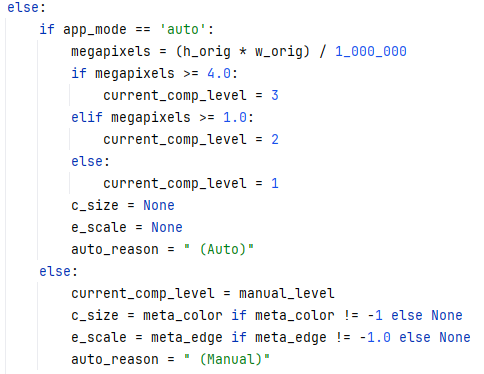
\includegraphics[width=0.5\textwidth]{media/images/code_smart_route.png}
    \caption{Реализация программного маршрутизатора (Smart Router)}
    \label{fig:code_smart_route}
\end{figure}

\subsection{Программная реализация каскадного вейвлет-кодера}

Модуль декомпозиции реализован в классе WaveletCompressor. Предложенный алгоритм представляет собой кастомный двухслойный конвейер сжатия, сочетающий математическую декомпозицию и транспортную контейнеризацию.

На первом слое выполняется дискретное вейвлет-преобразование на базе фильтра Хаара. Для обеспечения математически точной декомпозиции применяется специализированная библиотека PyWavelets (pywt), которая производит разделение цветовых каналов и извлекает аппроксимирующую LL-субполосу, уменьшая пространственное разрешение изображения в геометрической прогрессии на каждом уровне каскада.

На втором слое полученный вейвлет-скелет упаковывается в транспортный контейнер JPEG с эмпирически подобранным параметром качества 85\%. Выбор данного формата обусловлен необходимостью использования надежного алгоритма Хаффмана для упаковки байтов и обеспечения кроссплатформенности. В отличие от стандарта JPEG 2000, требующего сложных вычислительных мощностей для декодирования EBCOT-потока, предложенная схема использует JPEG исключительно как транспортную коробку для эффективной доставки низкочастотных данных нейросети. Реализация данного конвейера представлена на рисунке~\ref{fig:code_wavelet}.

\begin{figure}[ht]
    \centering
    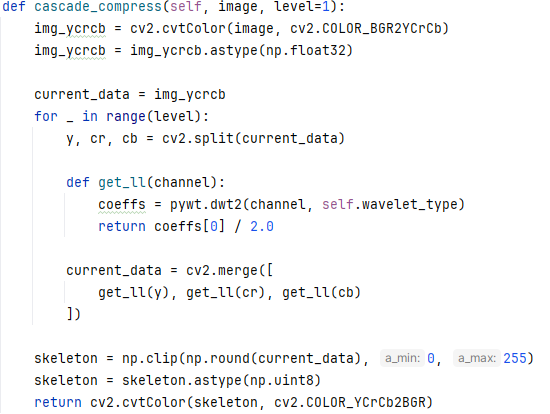
\includegraphics[width=0.5\textwidth]{media/images/code_wavelet.png}
    \caption{Математическая экстракция LL-субполосы и упаковка в контейнер}
    \label{fig:code_wavelet}
\end{figure}

\subsection{Реализация модуля экстракции гибридных метаданных}

Извлечение структурно-цветовых векторов реализовано в классе MetadataEngine и выполняется параллельно с вейвлет-декомпозицией. Метод экстракции цвета динамически высчитывает размер паспорта, выполняя сжатие для усреднения хроматики.

Для экстракции контуров изображение конвертируется в градации серого и к нему применяется оператор cv2.Canny \cite{canny1986}. Полученная бинарная маска также сжимается для минимизации сетевой нагрузки. Программная реализация методов извлечения представлена на рисунке~\ref{fig:code_metadata}.

\begin{figure}[ht]
    \centering
    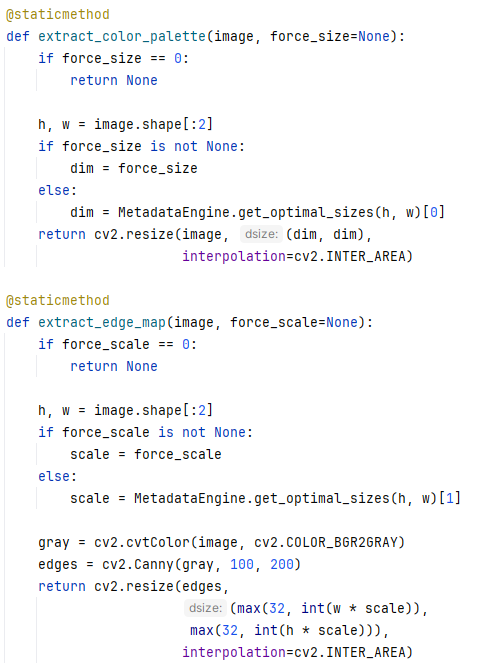
\includegraphics[width=0.5\textwidth]{media/images/code_metadata.png}
    \caption{Алгоритм экстракции цветового паспорта и карты границ}
    \label{fig:code_metadata}
\end{figure}

\subsection{Программная реализация нейросетевого апскейлинга и тайлинга}

Задачу реконструкции высокочастотных деталей выполняет класс AIEnhancer. Для повышения эффективности восстановления в классе реализован механизм автоматического выбора нейросетевой модели на основе анализа визуальной сложности входного кадра. Выбор осуществляется путем расчета дисперсии оператора Лапласиана, что позволяет оценить уровень детализации сцены. При высоком коэффициенте детализации (дисперсия превышает эмпирический порог 150) используется модель FSRCNN \cite{dong2016fsrcnn}, обладающая глубокой архитектурой для качественного восстановления микротекстур. Для изображений с преобладанием плавных градиентов применяется модель ESPCN \cite{shi2016}, эффективно работающая с субпиксельной сверткой и предотвращающая артефакты на однородных участках.

Инференс выбранных моделей осуществляется через подмодуль dnn\_superres, встроенный в OpenCV. Модели настраиваются на использование процессора (DNN\_TARGET\_CPU), что гарантирует кроссплатформенную работу сервера без требования наличия дискретного графического ускорителя.

Ввиду ограничений оперативной памяти реализован механизм тайловой маршрутизации (Overlapping Tiling). Изображение разбивается на блоки с нахлестом в 16 пикселей. Каждый тайл проходит через функцию восстановления. Краевые пиксели отсекаются для предотвращения артефактов свертки, а центральные части копируются в итоговую матрицу. Сразу после выполнения инференса модуль осуществляет предварительную цветовую коррекцию: выравнивание средних значений каналов в пространстве LAB. Это необходимо для базовой компенсации собственного цветового сдвига (color shift) нейросетей перед передачей тензора на этап семантической рекомбинации. Инициализация сети и метод инференса приведены на рисунке~\ref{fig:code_ai_engine}.

\begin{figure}[ht]
    \centering
    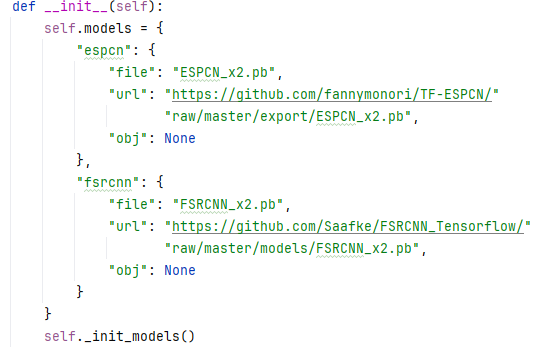
\includegraphics[width=0.5\textwidth]{media/images/code_ai_engine.png}
    \caption{Инициализация нейронной сети и тензорный инференс}
    \label{fig:code_ai_engine}
\end{figure}

\subsection[Семантическая постобработка и алгоритмы метрического\protect\\ контроля]{Семантическая постобработка и алгоритмы метрического контроля}

Финальный этап рекомбинации выполняется методами класса MetadataEngine. В ходе разработки было учтено, что при инкапсуляции вейвлет-скелета в транспортный контейнер JPEG происходит субдискретизация хроматических каналов (формат 4:2:0). Этот процесс, совместно с рекурсивным нейросетевым инференсом, вносит необратимые искажения в распределение яркости и цвета, что делает изображение визуально деградировавшим.

Для устранения данной проблемы реализован алгоритм цветовой коррекции в пространстве LAB на основе метода Рейнхарда \cite{reinhard2001}. Программа сопоставляет статистические моменты (среднее значение и стандартное отклонение) восстановленного изображения и переданного цветового паспорта по всем трем каналам (L, a, b). Математическая компенсация позволяет комплексно восстановить как исходную яркость, так и истинную хроматику пикселей без использования альфа-блендинга, предотвращая феномен нейросетевого галлюцинирования цвета.

Контурно-зависимое повышение резкости (Unsharp Mask) реализовано с использованием мягкой альфа-маски, которая формируется путем размытия бинарной карты Кенни фильтром Гаусса. Это обеспечивает бесшовное градиентное наложение резкости только на контуры объектов, исключая усиление шума на гладких поверхностях. Готовый кадр сохраняется в контейнер JPEG с коэффициентом качества 95\%.

Процесс объективной оценки качества реконструкции локализован в отдельном модуле. Расчет PSNR выполняется встроенной функцией cv2.PSNR. Для вычисления SSIM \cite{wang2004ssim} применяется функция structural\_similarity из библиотеки skimage.metrics \cite{scikit-image}. Интеграция данных модулей формирует законченную архитектуру асимметричного гибридного кодека.